\chapter{代码实现}

\section{相关技术}
    \subsection{NLP}

        由于规则检查中设计到大量的自然语言处理的部分,我们将其独立开发为一个模块nlputils.py。其对外提供了所有关于自然语言处理的接口。

        包括:
        
        parse\_sentence(sentence),输入参数为一个类型为字符串的句子,输出(返回值)为3个字符串的列表,分别表示句子中的主语、谓语动词和宾语。
        
        get\_verbs\_count\_of\_sentense(sentence),输入参数为一个类型为字符串的句子,输出(返回值)为4个字符串的列表,分别表示句子中的代词、副词、情态动词、分词。
        
        parse\_sentense\_tense(sentence),
        输入参数为一个类型为字符串的句子,输出(返回值)为一个字符串,表示该句子的时态:
        
        present 现在时
        
        past 过去时
        
        future 将来时
        
        none 其他
        
        parse\_word\_tense(sentence),
        输入参数为一个类型为字符串的单词,输出(返回值)为一个字符串,表示该单词的时态:
        
        present 现在时
        
        past 过去时
        
        future 将来时
        
        none 其他
        
        parse\_word\_type(sentence),
        输入参数为一个类型为字符串的单词,输出(返回值)为一个字符串,表示该单词的类型:
        
        verb 动词
        
        noun 名词
        
        adj 形容词
        
        none 其他

    \subsection{BFS}

        在处理句子时,使用nlp工具可以获得句子的每个单词的成分,句子的构成就成了一颗树,如图\ref{fig-coding-semantic-tree}所示:

        \begin{figure}
        \centering
        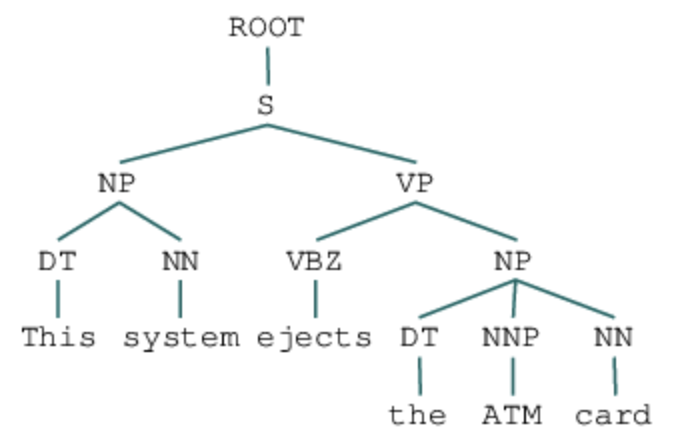
\includegraphics[width=5.76806in,height=3.80013in]{src/coding-semantic-tree.png}
        \caption{语义分析语法树}
        \label{fig-coding-semantic-tree}
        \end{figure}

        为了遍历到每个单词,我们采用广度优先搜索算法进行遍历。因为这样可以保证相同层的节点被顺序遍历到。

\section{开发协作流程}
    \subsection{GIT}
    本项目的开发协作使用git进行版本控制,并将repo放在GitHub上完全开源:\href{https://github.com/zen1995/rucmChecker}{\emph{rucmChecker}}。

    开发主要以2个分支的形式进行,一个master,一个lby。主要功能在master上开发,检查规则的功能在lby上开发,为了避免最后合并时冲突过多,lby分支在开发过程中会不断merge master上的更新。最后在合并分支时,我们选择集体编程这一模式。所有成员坐在一起,快速处理合并带来的冲突和bug,在2小时内完成合并任务,获得了可以正确运行的代码。在之后的bug修复、功能添加和测试时,所有的成员都在master上工作,不再使用新的分支。所有的commit和分支的历史信息,都可以在GitHub上找到,方便我们控制代码的所有版本,在必要时进行回退。并且知道每一行代码的修改者,在遇到bug或疑问时可以快速找到源头,进而解决。
    \subsection{分模块开发}
    根据设计,我们将所有的代码分为2大块:
    \begin{enumerate}
        \item
        项目核心的规则检查部分
        \item
        其它辅助部分,包括规则和rucm的加载,错误报告,参数处理,GUI交互等内容
    \end{enumerate}


    实际开发过程中,首先,架构师同学先根据类图写好框架,把所有需要的类定义出来,其相应的方法和属性也都写好,参数含义、类型,返回值含义、类型也都通过typing包或者名字、注释规定清楚。然后,程序员再开始分为2波,各自负责一块代码。当所有模块都开发完成后,所有人聚在一起,合并模块和代码,处理冲突和bug。事实证明,这种合作开发方式是十分高效和舒适的。大家各司其职,减少了大量开会和讨论的时间。合并完成后,测试人员进行测试,发现bug后,通过git的commit信息追踪到产生bug的程序员,将修复bug的任务交付给他。
\section{问题与解决办法}
    \subsection{NLP Server}
    nlp函数都依赖于nltk库和一个用于自然语言处理的Java\ server。开发过程中,最开始我们启动本地的server完成了代码。但在不同程序员完成各自模块,大家开始合并的时候,发现这样的设计并不友好。一方面,有些程序员并不能在本地顺利地配置好Java环境,启动本地server;另一方面,如果最后展示的时候程序还要依赖本地的server的话,还要给用户多加一步配置Java环境,启动server的步骤。经过讨论和商议,改为了在校园网的一台机器上启动这个server,24小时监听,程序默认会访问这个server,同时,给出一个参数-\/-url,即server的链接。允许用户自己配置server。这在对于校园网外的用户和需要自己内部使用server的用户还说也是可以接受的。而在最后的GUI版本中,我们经过一段时间的试用基本确定了校园网内通过网络服务器提供NLP处理的稳定性与可用性,因此对用户屏蔽了这些负责的设置内容,直接配置为固定的远程NLP服务。
    \subsection{复杂规则的实现}
    在实现和测试过程中,我们发现原有的设计并不能完全实现所有的规则检查。对于一些可以实现的规则,我们选择了修改原有设计,比如,在最开始的设计中,句子这个类并没有代词数量这一属性,但只有有了这个属性,一条规则才能很方便的实现。出现这种情况的原因在于,设计时虽然尽可能考虑所有的规则和情况,但毕竟抽象程度还是高于实现的,所有有些设计并不与实现完全对等。由于原来设计的低耦合性,在修改设计后,代码的修改和更新是十分迅速的。对于另外一些无法实现或没有必要实现的规则,我们选择在说明书中会陈述清楚,暂时不支持这些规则的检查。这样可以快速地生成可以交付给用户使用的版本,对于一些瑕疵选择之后的版本再解决,更加符合敏捷开发的原则。
    \subsection{中文适配}

    在第一次的展示中,吴老师给出要增加可以处理rucm中出现中文的情况,并检查其他组的rucm文件作为目标。
    增加对中文的适配,难度主要有2点:
    
    \begin{itemize}
        \item RUCM manual中,所有26条规则的定义和示例都是针对英文的,完全没有考虑中文。比如,对于第15条规则,中文中并不存在分词。所以我们需要重新定义26条默认规则,删除不必要和不方便实现的默认规则。
        \item 中文NLP技术与英文的差别还是很大的,尤其是语法分析部分,句子成分和词性区别很大。很多函数需要准备2套规则,分别适应于不同的语言。对于一个句子中可能同时出现中英文的情况,比如有些同学的rucm文件的关键字和名词用英文,其他地方使用中文,对于这种情况,我们经过讨论决定,不予支持。即不允许中英文在一个句子里混杂,但是允许不同句子使用不同的语言。
    \end{itemize}

    中文NLP主要借助了2个工具:结巴分词 和 Standford parser for Chinese。
    其中,结巴分词主要用于,对中文进行分词,和词性分析。
    Standford parser for Chinese用于中文的语法分析。
    工具的选择主要考虑到开发速度、易用性和准确性。英文中不存在分词问题,每个单词都是以空格分隔的。但中文中,分词确实被广泛研究的,是一切NLP的基础。经过调研,“结巴分词”使用率最广。我们选择使用“结巴分词”作为我们的分词工具和词性分析工具。
    结巴分词并不提供更高级的NLP技术。对于语法分析,我们仍然选择Stanford 的parser。主要考虑是,Standford parser for Chinese的接口和使用方法与Stanford parser for English相同。直接使用它可以降低学习成本,提高开发效率。

    针对可能出现的中英文混杂,我们实现了自动切换分析工具的功能。即根据句子的语言类别,使用2套不同的函数进行分析、NLP处理。降低了用户使用的难度,提高了可用性。
    